\section{CNN Classifier}

\subsection{Region of Interest Size}

From the skeletons we generate locations in the center of potential merges. 
We extract a cubic region of interest around each location.
We experimented with three different region of interest side lengths: $800 \textrm{nm}$, $1200 \textrm{nm}$, and $1600 \textrm{nm}$. 
Side lengths of $1600 \textrm{nm}$ performed better on the training and validation data on our network. 

\subsection{CNN Parameters}

We experimented with several different network architectures before deciding on the one presented in our paper. 
We considered stochastic gradient descent with Nesterov momentum and the Adam optimizer.
In addition we toggled between a binary cross entropy and mean squared error loss function.
Also, we considered four varying input sizes that corresponding to different cube sizes output from the final max pooling layer. 
After running a brute force search over all of these possible architectures, we found that the best architecture used a SGD optimizer with Nesterov momentum, a mean squared error loss function, and an input size of $76 \times 76 \times 24$. 

\subsection{Architecture}

\begin{figure*}
	\centering
	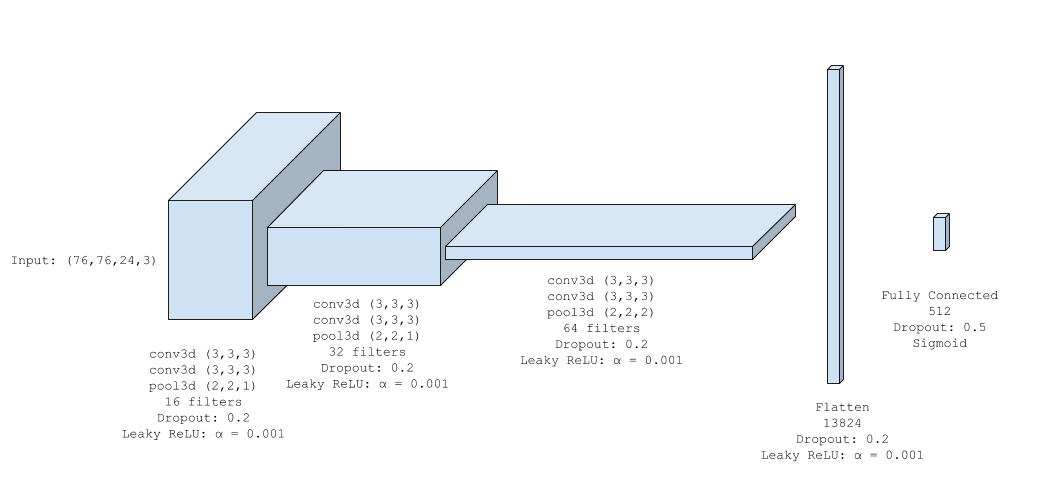
\includegraphics[width=0.9\linewidth]{./figures/architecture.png}
	\caption{The final architecture presented in this paper.}
	\label{fig:architecture}
\end{figure*}

Figure \ref{fig:architecture} shows the final architecture that produced the best results on the validation data. 
The input data was $76 \times 76 \times 24$ voxels in size with $3$ channels per voxel. 
This corresponds to an output size from the third layer of double convolution of $6 \times 6 \times 6$. 
This flattens to a vector of size $13,824$ which enters a dense layer of output size $512$ followed by another dense layer of output size $1$. 
All activation layers are Leaky ReLU with $\alpha=0.001$ except for the final layer which has a sigmoid activation layer.